\documentclass{journal}
\usepackage{graphicx}	% package for using graphics
\usepackage{float}	% package for positioning figures

\title{AIRFRAME ANALYSIS}

\author{Nathan Pettit}


\begin{document}
	
	\maketitle	
	
	\section{Introduction}
	
	This report covers research done on airframes using the VortexLattice.jl library, specifically how aspect ratio and efficiency are related, how tail volume ratios affect stability derivatives, and how angle of attack affects the lift coefficient. A wiki with unfamiliar terms and their corresponding equations and figures can be found at the end of this report.
	
	\section{Methods}
	The results of this research came from evaluating airframes using VortexLattice.jl, as well as writing new functions to help in evaluating the airframes. There were 4 functions that were  used:
	
	\begin{enumerate}
		\item aoa\_effect() - this evaluated airframes and calculated their coefficient of lift for varying angles of attack 
		\item wing\_efficiency() - this calculated the efficiency of airframes with varying aspect ratios; it did this by calculating the lift and drag coefficients for every aspect ratio
		\item stability\_derivatives() - this calculated the stability derivatives for airframes with different horizontal and vertical tail ratios
		\item vortex\_lattice() - this was the main function that performed all the necessary VortexLattice calculations for the other functions 
	\end{enumerate}
	
	\section{Results and Discussion}
	
	\subsection{Aspect Ratio vs. Efficiency}
	
	In order to see the relationship between aspect ratio and the efficiency, the wing\_efficiency() function was used. When it was run, it calculated the inviscid span efficiency (see equation \ref{eqn:efficiency}) for airframes with aspect ratios (see equation \ref{eqn:aspect-ratio}) ranging from 3 to 15.
	
	\begin{equation}
		e_{inv} = \frac{C_L^2}{\pi{ARC_D}}
		\label{eqn:efficiency}
	\end{equation}

	\begin{equation}
		AR = \frac{b}{c} = \frac{b^2}{S_{ref}}
		\label{eqn:aspect-ratio}
	\end{equation}
	
	After the program calculated the efficiency, it produced a plot shown in figure \ref{fig:efficiency}. \\
	
	\begin{figure}[H]
		\centering
		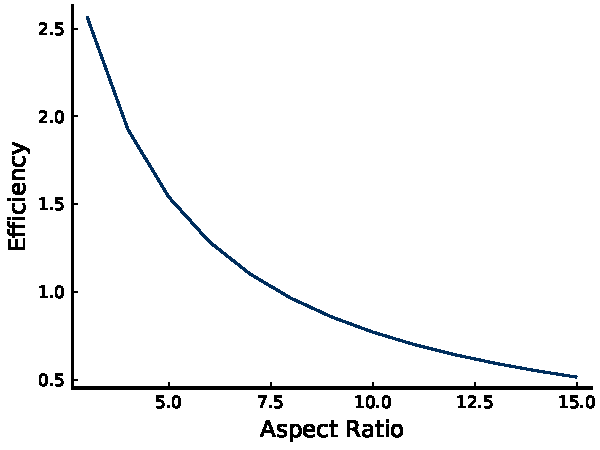
\includegraphics{../graphics/efficiency.pdf}
		\caption{\emph{This diagram shows the relationship between aspect ratio and inviscid span efficiency.}}
		\label{fig:efficiency}
	\end{figure}

	In reality, there is actually no physical relationship between an airframe's aspect ratio and its efficiency, but figure \ref{fig:efficiency} does mathematically plot it correctly. However, that plot is simply the definition of inviscid span efficiency. \\
	
	\subsection{Tail Volume Ratios vs Stability Derivatives}
	
	Another characteristic of these airframes that was observed was their stability derivatives. Stability derivatives were calculated for airframes with different tail volume ratios, both vertical and horizontal. The definitions of those ratios are equations \ref{eqn:vtail-ratio} and \ref{eqn:htail-ratio}. The stability derivatives that are affected by a change in vertical tail volume ratio are \(C_{\ell{b}}\) and \(C_{nb}\). \(C_{\ell{b}}\) is the stability derivative associated with roll stability. \(C_{nb}\) is the stability derivative associated with yaw stability. An airframe is stable if \(C_{\ell{b}}\) is less than 0 and \(C_{nb}\) is greater than 0. \\
	
	\begin{equation}
		V_v = \frac{l_vS_v}{Sb}
		\label{eqn:vtail-ratio}
	\end{equation}
	
	\begin{equation}
		V_h = \frac{l_tS_t}{SC_{ma}}
		\label{eqn:htail-ratio}
	\end{equation}

	In figure \ref{fig:vtail-stability} , we can see that the airframe is stable for vertical tail volume ratios greater than 0.003, but it becomes unstable when the ratio is less than 0.003, at around 0.002. The stability derivatives that are affected by a change in horizontal tail volume ratio are \(C_{La}\) and \(C_{ma}\). An airframe is stable if \(C_{La}\) is greater than 0 and \(C_{ma}\) is less than 0. Figure \ref{fig:htail-stability} shows that the airframe is stable for horizontal tail volume ratios greater than 0.05, but becomes unstable when the ratio is less than 0.05, at around 0.025. \\
	
	\begin{figure}[H]
		\centering
		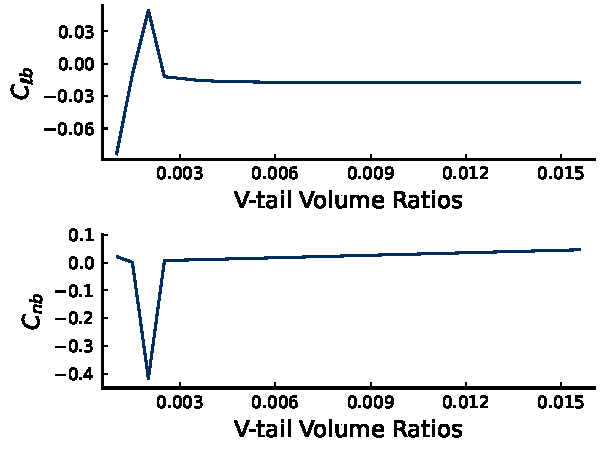
\includegraphics[scale=0.73]{../graphics/vtail-stability.pdf}
		\caption{\emph{This diagram shows the relationship between vertical tail volume ratio, \(C_{\ell{b}}\), and \(C_{nb}\).}}
		\label{fig:vtail-stability}
	\end{figure}

	\begin{figure}[H]
		\centering
		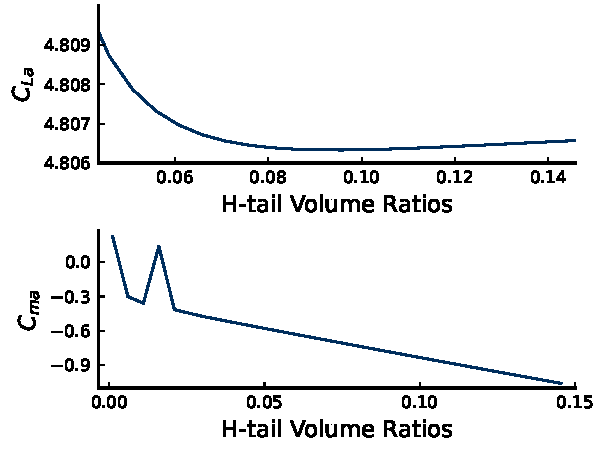
\includegraphics[scale=0.73]{../graphics/htail-stability.pdf}
		\caption{\emph{This diagram shows the relationship between horizontal tail volume ratio, \(C_{La}\), and \(C_{ma}\).}}
		\label{fig:htail-stability}
	\end{figure}
	
	These ratios are arbitrary and will be different among models, but they are still extremely important. \\
	
	\subsection{Angle of attack vs lift coefficient}
	
	In previous research about airfoils, I found that as angle of attack increases, the lift coefficient also increases, up to a certain point. At that point, the lift coefficient sharply drops, and this is where stall takes place. In that previous research, Xfoil.jl was used to calculate the lift coefficient for varying angles of attack. A relationship between angle of attack and lift was also tried to be found here, but instead of using Xfoil.jl, VortexLattice.jl was used. A plot was produced showing the relationship between angle of attack and lift (see figure \ref{fig:aoa-lift}). \\
	
	\begin{figure}[H]
		\centering
		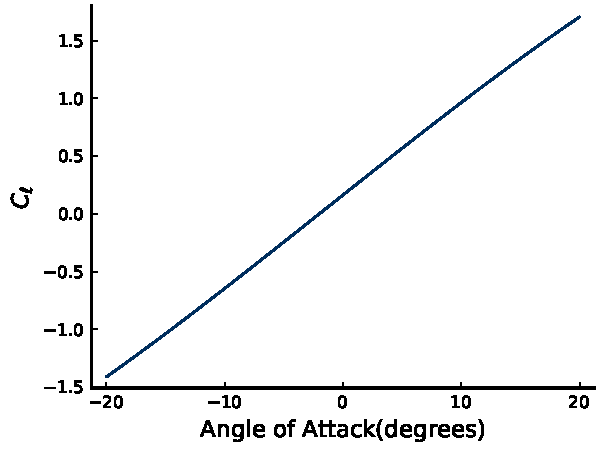
\includegraphics{../graphics/aoa-lift.pdf}
		\caption{\emph{This diagram shows the relationship between angle of attack and lift for an airframe.}}
		\label{fig:aoa-lift}
	\end{figure}

	In comparison to the plot created using Xfoil.jl, figure \ref{fig:aoa-lift} looks very similar between angles of attack of -10 and 10. However, past those angles of attack is where it differs. In the Xfoil plot, it shows very clearly where stall would take place, but in this VortexLattice plot, the plot continues linearly and never drops off, never indicating stall. This is why the Vortex Lattice method is not always a great choice for investigating airframes. It is only accurate when the angle of attack is small, because it assumes that the flow is inviscid at all angles of attack. This is why in figure \ref{fig:aoa-lift} it looks very linear and doesn't indicate where stall would take place, where as the Xfoil plot does.
 	
	\section*{Appendix}
	
	\begin{itemize}
		\item Sweep: the angle at which the wing is translated backwards (or occasionally forwards) relative to the root chord of the wing (see figure \ref{fig:sweep})
		
		\begin{figure}[H]
			\centering
			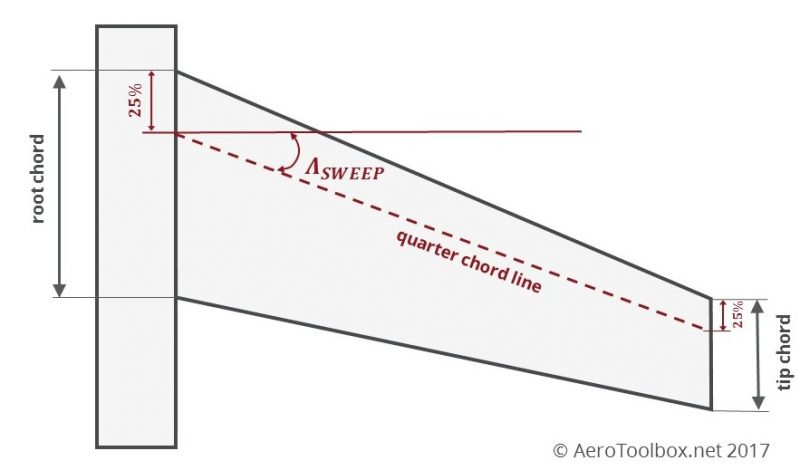
\includegraphics[scale=0.4]{../graphics/sweep.jpg}
			\caption{\emph{This diagram shows what sweep is on an airframe.}}
			\label{fig:sweep}
		\end{figure}
		
		\item Aspect Ratio: aspect ratio of a wing is the ratio of its span to its mean chord. It is equal to the square of the wingspan divided by the wing area. Thus, a long, narrow wing has a high aspect ratio, whereas a short, wide wing has a low aspect ratio (see equation \ref{eqn:aspect-ratio-wiki})
		
		\begin{equation}
			AR = \frac{b}{c} = \frac{b^2}{S_{ref}}
			\label{eqn:aspect-ratio-wiki}
		\end{equation}
	
		\item Wake Vortex/Tip Vortex: a lifting wing has higher pressure on the bottom surface as compared to the top, and so fluid will circulate around the tips (see figure \ref{fig:downwash-wakevortex})
		\item Downwash: can be viewed more fundamentally as a consequence of Newton’s third law. If a body is producing lift, colloquially we might say that means that the air is pushing the body up. Thus, by Newton’s third law, the body must be pushing the air downward. Thus, any three-dimensional lifting body will leave behind a wake of downward moving air (see figure \ref{fig:downwash-wakevortex})
		
		\begin{figure}
			\centering
			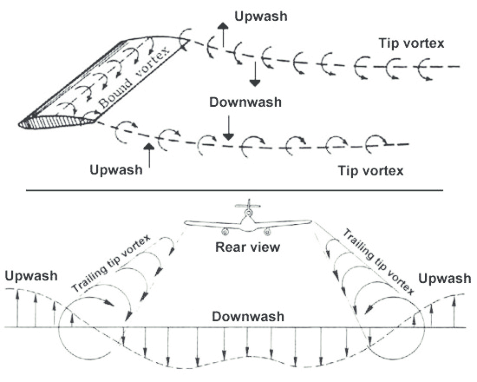
\includegraphics[scale=0.4]{../graphics/downwash-wakevortex.png}
			\caption{\emph{This diagram shows how downwash and wake vortexes are formed.}}
			\label{fig:downwash-wakevortex}
		\end{figure}
	
		\item Induced Drag/Vortex Drag: major consequence of this downwash, is that energy is left behind in the wake. Or in other words, the wing produces drag
		\item Inviscid Span Efficiency:  the inviscid span efficiency could be considered a measure of how close the lift distribution is to elliptic. All planar distributions will have \(e_{inv} <= 1\). A nonplanar lift distribution (e.g., adding winglets) can increase the inviscid span efficiency above 1 (see equation \ref{eqn:efficiency-wiki})
		
		\begin{equation}
			e_{inv} = \frac{C_L^2}{\pi{ARC_D}}
			\label{eqn:efficiency-wiki}
		\end{equation}
	
		\item Vortex Filament: an arbitrary vortex line segment
		\item Vortex Lattice Method: an extension of thin airfoil theory into three dimensions
		\item Tail Volume Ratio: relates the shape of the tail to the wing 
		\subitem Vertical Tail Volume Ratio: 
		
		\begin{equation}
			V_v = \frac{l_vS_v}{Sb}
			\label{eqn:vtail-ratio-wiki}
		\end{equation}
	
		\subitem Horizontal Tail Volume Ratio:
		
		\begin{equation}
			V_h = \frac{l_tS_t}{SC_{ma}}
			\label{eqn:htail-ratio-wiki}
		\end{equation}
	
		\item Stability Derivatives: measures of how particular forces and moments on an aircraft change as other parameters related to stability change
		
	\end{itemize}
	
	
\end{document}
